\documentclass[10pt]{article}

\usepackage{graphicx}
\usepackage{hyperref}

\begin{document}

\title{COP290: Assignment-2 Documentation}
\author{\\ N.Manoj Devender : 2013CS10240\\K.V.Hemanth : 2013CS10233\\Gursharanpreet singh : 2013CS10222\\Homesh Rawat :2013CS10226
}
\date{\ 24-3-2015}
\maketitle

\hypersetup{
    colorlinks=true,
    linkcolor=blue,
    filecolor=magenta,      
    urlcolor=cyan,
}
\tableofcontents

\newpage 
\section{Design of SniperLeague}
     Our game SniperLeague is designed in various modules to enable efficient code management and debugging. The following is the list of modules designed in the implementation of it.

\section{Sub Components in Design of SniperLeague}

\subsection*{SCREEN SHOT OF THE GAME:}
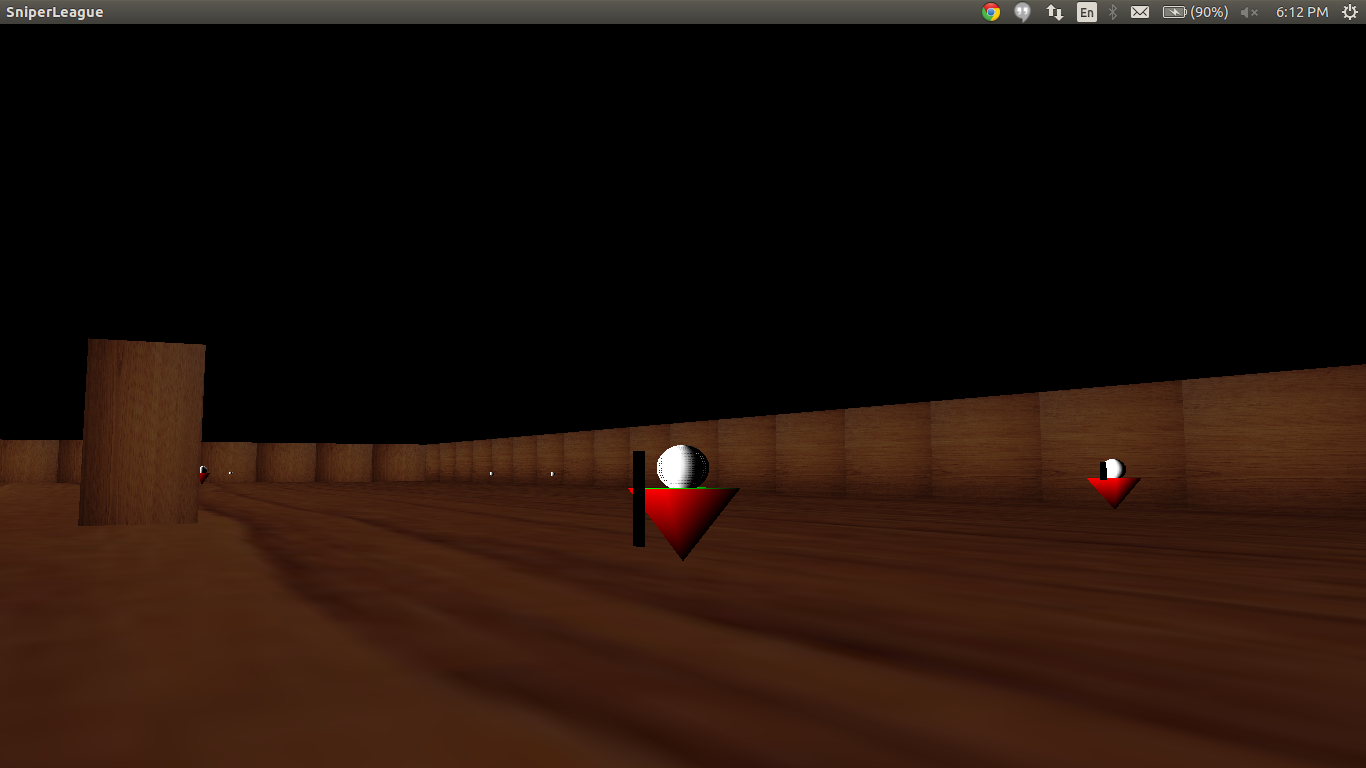
\includegraphics[width=\textwidth]{screen_shot.png}
\\
\subsection{GAME PLAN:}
 \textbf{3D Action Game}\\ It is a 3D Shooting action game.
Each Player has a health bar and infinite number of bullets.If player gets shot then his/her health bar would be decreased. Once the health bar is completely over the player dies. 
Maximum number of players limit is M ( M = 4 ).
Each player can move in any direction.
Players can change their location within the boundaries of the field.
In the field, there are rigid walls for hiding during an attack. Bullets can be fired in any direction by left clicking the mouse. 
\\
\\
\\
\\
\\

	\subsection{GUI}
     SFML and opengl is used in creating the client GUI interface.\\\\ 
     \textbf{User Options:}
	 The user will be getting below options while using the application:  \\
	\subsubsection{Host my newgame:}
			  One player initiates a new game instance on the server and is hereby referred to as the ‘admin’. Player can start a new game by giving the port number and I.P address to instantiate the server.

	\subsubsection{Join the game:}
                         Players can join he existing hosted game by keying in server ip,server port number and his own port number

	\subsubsection{TYPE OF GAME:}
	         Every player gets choice to select between Multiplayer game or single player game. Based upon his choice, a new game would be created.  
    \subsubsection{MOTION:}
    A Player can move in any direction using arrow keys and mouse.He can shoot in the direction of the mouse pointer's click. Walls will absorb the bullets.
	\subsubsection{NUMBER OF BOTS:}		
  At the initiation of a Single player new game itself the player is asked How many bots does he wants to face during the game. Accordingly, the artificial robots are placed in the game. The maximum number of bots that can be generated are 3 in a game.\\
There is a \emph{Readme.txt} file in order to make the user aware of the usage in-case of any ambiguity.
\subsection{GAME GRAPHICS:}
    The players and the game environment are drawn by programming OpenGL in c++. We used the basic structures, textures, inbuilt functions of the OpenGL in creation of body of player,obstacles,walls and other necessary elements of game.

\subsection{NETWORKING:}
UDP is used as our networking method.
After every 't' time the packages will be exchanged between the players.
Every package has player id and sequence number enclosed in it.
Whenever the player receive the package of other player then the former will send the acknowledgment package of the same sequence number  and if latter doesn’t receive the acknowledgment package within some time then he sends the package again.
If a player gets disconnected during the game then the game will still go on for other players however this player will still try to send and receive the packages from other players. However if the player doesn't send any acknowledgment packages or his own packages for some time then the player will be disconnected permanently. But the probability of this happening is very low as each player is sending and receiving data from every other player.
\\

\subsection*{ NETWORK MODEL:}

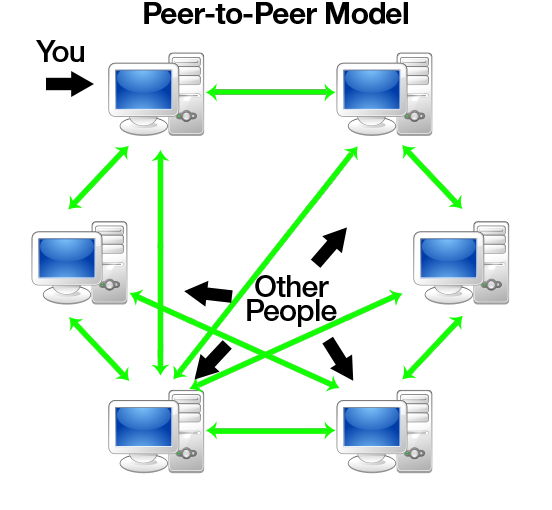
\includegraphics[width=\textwidth]{pto1.png}
\\
\\
Initially our game is created by a server with whom the other players will be connected. After all the players has been created then the server will send the addresses of every player to every other player thus setting up a p2p server.
\\
\subsection{SYNCHRONISATION OF DATA:}
In order to keep the simulation accurate, every peer is responsible for propagating only the information about its ship, not the others. This means that, if the game has four players - say A, B, C and D - player A is the only one able to inform about where ship A is, whether it got hit or if it fired a bullet , and so on.  All other players will receive messages from A, informing about his actions and they will react accordingly, so if A's bullet got C's ship, then C will broadcast a message informing it was hit.\\

\subsection*{BASIC AI LOGIC:}
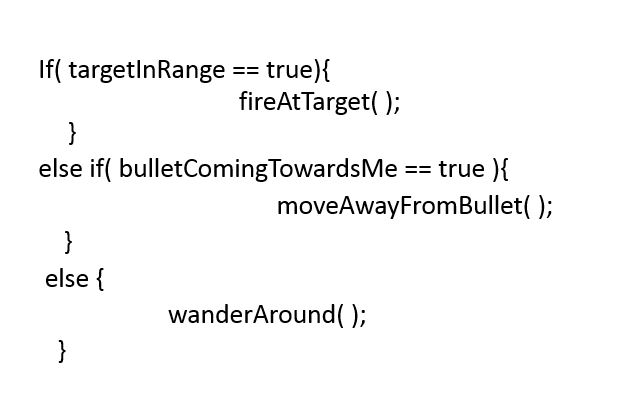
\includegraphics[width=\textwidth]{AI.jpg}
\\
\subsection{ARTIFICIAL INTELLIGENCE:}
We simulated intelligence in each of individual units rather than a single intelligence unit. We will apply different AI logics for different "states" of the player. We need to maximize the life expectancy of the bot. To compute the expected score for any action all possible moves and weight of the possible outcome with the probability of the player doing that move will be used. 
\\
\section{TestCases:}
First we will be testing the UDP network without any GUI (just sending and receiving the messages)
Then we start with GUI and we will make the necessary algorithms for player motion and shooting.
Then we will test our game for 2 or more players (no bot) 
Then we will implement AI algorithms for bot.
 Finally we will test our game with all the components.
\\

\end{document}


